
%%--------------------------------------------------
%% Serway: Physics for Scientists and Engineers
%%--------------------------------------------------


%% Chapter 06: Circular Motion and other
%%     Applications of Newton's Laws
%%--------------------------------------------------


%% Table of Contents
%%--------------------------------------------------

%% 6.1 Newton's Second Law for a Particle in Uniform Circular Motion
%% 6.2 Nonuniform Circular Motion
%% 6.3 Motion in Accelerated Frames
%% 6.4 Motion in the Presence of Resistive Forces


%% Serway Multiple Choice Questions
%%--------------------------------------------------
\element{serway-mc}{
\begin{question}{serway-ch06-q01}
    A race car travels \SI{40}{\meter\per\second} around a banked (\ang{45} with the horizontal)
        circular (radius = \SI{0.20}{\kilo\meter}) track. 
    What is the magnitude of the resultant force on the \SI{80}{\kilo\gram} driver of this car?
    \begin{multicols}{3}
    \begin{choices}
        \wrongchoice{\SI{0.68}{\kilo\newton}}
      \correctchoice{\SI{0.64}{\kilo\newton}}
        \wrongchoice{\SI{0.72}{\kilo\newton}}
        \wrongchoice{\SI{0.76}{\kilo\newton}}
        \wrongchoice{\SI{0.52}{\kilo\newton}}
    \end{choices}
    \end{multicols}
\end{question}
}

\element{serway-mc}{
\begin{question}{serway-ch06-q02}
    An airplane travels \SI{80}{\meter\per\second} as it makes a horizontal
        circular turn which has a \SI{0.80}{\kilo\meter} radius. 
    What is the magnitude of the resultant force on the
        \SI{75}{\kilo\gram} pilot of this airplane?
    \begin{multicols}{3}
    \begin{choices}
        \wrongchoice{\SI{0.69}{\kilo\newton}}
        \wrongchoice{\SI{0.63}{\kilo\newton}}
        \wrongchoice{\SI{0.66}{\kilo\newton}}
      \correctchoice{\SI{0.60}{\kilo\newton}}
        \wrongchoice{\SI{0.57}{\kilo\newton}}
    \end{choices}
    \end{multicols}
\end{question}
}

\element{serway-mc}{
\begin{question}{serway-ch06-q03}
    An airplane moves \SI{140}{\meter\per\second} as it travels around a vertical circular loop which has a \SI{1.0}{\kilo\meter} radius. 
    What is the magnitude of the resultant force on the \SI{70}{\kilo\gram} pilot of this plane at the bottom of this loop?
    \begin{multicols}{3}
    \begin{choices}
        \wrongchoice{\SI{2.1}{\kilo\newton}}
      \correctchoice{\SI{1.4}{\kilo\newton}}
        \wrongchoice{\SI{0.69}{\kilo\newton}}
        \wrongchoice{\SI{1.5}{\kilo\newton}}
        \wrongchoice{\SI{1.3}{\kilo\newton}}
    \end{choices}
    \end{multicols}
\end{question}
}

\element{serway-mc}{
\begin{question}{serway-ch06-q04}
    A car travels along the perimeter of a vertical circle
        (radius = \SI{0.25}{\kilo\meter}) at a constant speed of \SI{30}{\meter\per\second}. 
    What is the magnitude of the resultant force on the \SI{60}{\kilo\gram}
        driver of the car at the lowest point on this circular path?
    \begin{multicols}{3}
    \begin{choices}
        \wrongchoice{\SI{0.37}{\kilo\newton}}
        \wrongchoice{\SI{0.80}{\kilo\newton}}
      \correctchoice{\SI{0.22}{\kilo\newton}}
        \wrongchoice{\SI{0.59}{\kilo\newton}}
        \wrongchoice{\SI{0.45}{\kilo\newton}}
    \end{choices}
    \end{multicols}
\end{question}
}

\element{serway-mc}{
\begin{question}{serway-ch06-q05}
    A \SI{30}{\kilo\gram} child rides on a circus Ferris wheel that takes her
        around a vertical circular path with a radius of \SI{20}{\meter} every \SI{22}{\second}.
    What is the magnitude of the resultant force on the child at the highest point on this trajectory?
    \begin{multicols}{3}
    \begin{choices}
      \correctchoice{\SI{49}{\newton}}
        \wrongchoice{\SI{0.29}{\kilo\newton}}
        \wrongchoice{\SI{0.34}{\kilo\newton}}
        \wrongchoice{\SI{0.25}{\kilo\newton}}
        \wrongchoice{\SI{0.76}{\kilo\newton}}
    \end{choices}
    \end{multicols}
\end{question}
}

\element{serway-mc}{
\begin{question}{serway-ch06-q06}
    An amusement ride consists of a car moving in a vertical circle on the end of a rigid boom. 
    The radius of the circle is \SI{10}{\meter}. 
    The combined weight of the car and riders is \SI{5.0}{\kilo\newton}.
    At the top of the circle the car has a speed of \SI{5.0}{\meter\per\second}
        which is not changing at that instant. 
    What is the force of the boom on the car at the top of the circle?
    \begin{multicols}{2}
    \begin{choices}
        \wrongchoice{\SI{3.7}{\kilo\newton} (Down)}
        \wrongchoice{\SI{1.3}{\kilo\newton} (Down)}
        \wrongchoice{\SI{6.3}{\kilo\newton} (Up)}
      \correctchoice{\SI{3.7}{\kilo\newton} (Up)}
        \wrongchoice{\SI{5.2}{\kilo\newton} (Down)}
    \end{choices}
    \end{multicols}
\end{question}
}

\element{serway-mc}{
\begin{question}{serway-ch06-q07}
    A highway curve has a radius of \SI{0.14}{\kilo\meter} and is unbanked. 
    A car weighing \SI{12}{\kilo\newton} goes around the curve at a speed of \SI{24}{\meter\per\second} without slipping. 
    What is the magnitude of the horizontal force of the road on the car?
    \begin{multicols}{3}
    \begin{choices}
        \wrongchoice{\SI{12}{\kilo\newton}}
        \wrongchoice{\SI{17}{\kilo\newton}}
        \wrongchoice{\SI{13}{\kilo\newton}}
      \correctchoice{\SI{5.0}{\kilo\newton}}
        \wrongchoice{\SI{49}{\kilo\newton}}
    \end{choices}
    \end{multicols}
\end{question}
}

\element{serway-mc}{
\begin{question}{serway-ch06-q08}
    A \SI{4.0}{\kilo\gram} mass on the end of a string rotates in a
        circular motion on a horizontal frictionless table. 
    The mass has a constant speed of \SI{2.0}{\meter\per\second}
        and the radius of the circle is \SI{0.80}{\meter}.
    What is the magnitude of the resultant force acting on the mass?
    \begin{multicols}{3}
    \begin{choices}
        \wrongchoice{\SI{39}{\newton}}
      \correctchoice{\SI{20}{\newton}}
        \wrongchoice{\SI{44}{\newton}}
        \wrongchoice{\SI{0}{\newton}}
        \wrongchoice{\SI{30}{\newton}}
    \end{choices}
    \end{multicols}
\end{question}
}

\element{serway-mc}{
\begin{question}{serway-ch06-q09}
    A stunt pilot weighing \SI{0.70}{\kilo\newton} performs a vertical circular dive of radius \SI{0.80}{\kilo\meter}.
    At the bottom of the dive,
        the pilot has a speed of \SI{0.20}{\kilo\meter\per\second} which at that instant is not changing.
    What force does the plane exert on the pilot?
    \begin{multicols}{2}
    \begin{choices}
        \wrongchoice{\SI{3.6}{\kilo\newton} up}
      \correctchoice{\SI{4.3}{\kilo\newton} up}
        \wrongchoice{\SI{2.9}{\kilo\newton} down}
        \wrongchoice{\SI{2.9}{\kilo\newton} up}
        \wrongchoice{\SI{5.8}{\kilo\newton} down}
    \end{choices}
    \end{multicols}
\end{question}
}

\element{serway-mc}{
\begin{question}{serway-ch06-q10}
    A car travels around an unbanked highway curve
        (radius \SI{0.15}{\kilo\meter}) at a constant speed of \SI{25}{\meter\per\second}. 
    What is the magnitude of the resultant force acting on the driver,
        who weighs \SI{0.80}{\kilo\newton}?
    \begin{multicols}{3}
    \begin{choices}
        \wrongchoice{\SI{0.87}{\kilo\newton}}
      \correctchoice{\SI{0.34}{\kilo\newton}}
        \wrongchoice{\SI{0.80}{\kilo\newton}}
        \wrongchoice{\SI{0.00}{\kilo\newton}}
        \wrongchoice{\SI{0.67}{\kilo\newton}}
    \end{choices}
    \end{multicols}
\end{question}
}

\element{serway-mc}{
\begin{question}{serway-ch06-q11}
    A \SI{0.50}{\kilo\gram} mass attached to the end of a string swings in a vertical circle (radius = \SI{2.0}{\meter}).
    When the mass is at the lowest point on the circle,
        the speed of the mass is \SI{12}{\meter\per\second}.
    What is the magnitude of the force of the string on the mass at this position?
    \begin{multicols}{3}
    \begin{choices}
        \wrongchoice{\SI{31}{\newton}}
        \wrongchoice{\SI{36}{\newton}}
      \correctchoice{\SI{41}{\newton}}
        \wrongchoice{\SI{46}{\newton}}
        \wrongchoice{\SI{23}{\newton}}
    \end{choices}
    \end{multicols}
\end{question}
}

\element{serway-mc}{
\begin{question}{serway-ch06-q12}
    A roller-coaster car has a mass of \SI{500}{\kilo\gram}
        when fully loaded with passengers. 
    \begin{center}
    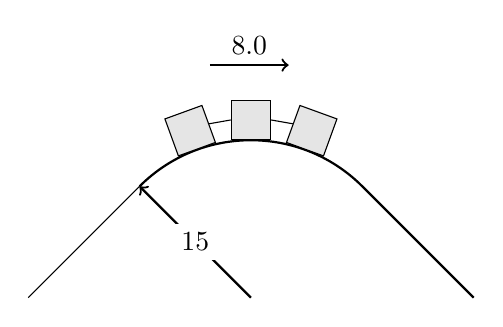
\begin{tikzpicture}
        \draw[thick] (135:2) arc (135:45:2) -- ++ (315:2);
        \node[fill=white!90!black,rectangle,anchor=south,rotate=+20,draw,minimum size=0.5cm] (A) at (110:2) {};
        \node[fill=white!90!black,rectangle,anchor=south,rotate=0,draw,minimum size=0.5cm] (B) at (90:2) {};
        \node[fill=white!90!black,rectangle,anchor=south,rotate=-20,draw,minimum size=0.5cm] (C) at (70:2) {};
        \draw (A.east) -- (B.west) (B.east) -- (C.west);
        \draw (135:2) -- ++ (225:2);
        \draw[thick,->] (0,0) -- (135:2) node[pos=0.5,anchor=center,fill=white] {\SI{15}{\meter}};
        \draw[thick,->] (100:3) -- ++(0:1) node[anchor=south,pos=0.5] {\SI{8.0}{\meter\per\second}};
    \end{tikzpicture}
    \end{center}
    The car passes over a hill of radius \SI{15}{\meter}, as shown. 
    At the top of the hill, the car has a speed of \SI{8.0}{\meter\per\second}.
    What is the force of the track on the car at the top of the hill?
    \begin{multicols}{2}
    \begin{choices}
        \wrongchoice{\SI{7.0}{\kilo\newton} up}
        \wrongchoice{\SI{7.0}{\kilo\newton} down}
        \wrongchoice{\SI{2.8}{\kilo\newton} down}
      \correctchoice{\SI{2.8}{\kilo\newton} up}
        \wrongchoice{\SI{5.6}{\kilo\newton} down}
    \end{choices}
    \end{multicols}
\end{question}
}

\element{serway-mc}{
\begin{question}{serway-ch06-q13}
    A \SI{0.20}{\kilo\gram} object attached to the end of a string swings in a vertical circle (radius = \SI{80}{\centi\meter}). 
    At the top of the circle the speed of the object is \SI{4.5}{\meter\per\second}. 
    What is the magnitude of the tension in the string at this position?
    \begin{multicols}{3}
    \begin{choices}
        \wrongchoice{\SI{7.0}{\newton}}
        \wrongchoice{\SI{2.0}{\newton}}
      \correctchoice{\SI{3.1}{\newton}}
        \wrongchoice{\SI{5.1}{\newton}}
        \wrongchoice{\SI{6.6}{\newton}}
    \end{choices}
    \end{multicols}
\end{question}
}

\element{serway-mc}{
\begin{question}{serway-ch06-q14}
    A roller-coaster car has a mass of \SI{500}{\kilo\gram} when fully loaded with passengers. 
    \begin{center}
    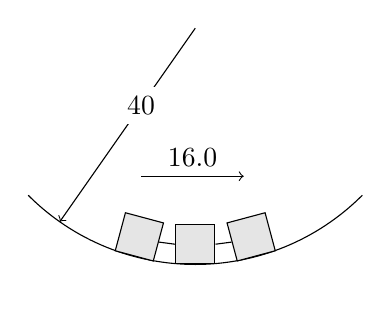
\begin{tikzpicture}
        \draw (225:3) arc (225:315:3);
        \draw[->] (0,0) -- (235:3) node[pos=0.4,fill=white,anchor=center] {\SI{40}{\meter}};
        \node[fill=white!90!black,rectangle,anchor=south,rotate=-15,draw,minimum size=0.5cm] (A) at (255:3) {};
        \node[fill=white!90!black,rectangle,anchor=south,rotate=0,draw,minimum size=0.5cm] (B) at (270:3) {};
        \node[fill=white!90!black,rectangle,anchor=south,rotate=+15,draw,minimum size=0.5cm] (C) at (285:3) {};
        \draw (A.east) -- (B.west) (B.east) -- (C.west);
        \draw[->] (250:2) -- ++(0:1.3) node[anchor=south,pos=0.5] {\SI{16.0}{\meter\per\second}};
    \end{tikzpicture}
    \end{center}
    At the bottom of a circular dip of radius \SI{40}{\meter} (as shown in the figure) the car has a speed of \SI{16}{\meter\per\second}. 
    What is the magnitude of the force of the track on the car at the bottom of the dip?
    \begin{multicols}{3}
    \begin{choices}
        \wrongchoice{\SI{3.2}{\kilo\newton}}
      \correctchoice{\SI{8.1}{\kilo\newton}}
        \wrongchoice{\SI{4.9}{\kilo\newton}}
        \wrongchoice{\SI{1.7}{\kilo\newton}}
        \wrongchoice{\SI{5.3}{\kilo\newton}}
    \end{choices}
    \end{multicols}
\end{question}
}

\element{serway-mc}{
\begin{question}{serway-ch06-q15}
    A \SI{0.50}{\kilo\gram} mass attached to the end of a string swings in a vertical circle (radius = \SI{2.0}{\meter}). 
    When the mass is at the highest point of the circle the speed of the mass is \SI{8.0}{\meter\per\second}. 
    What is the magnitude of the force of the string on the mass at this position?
    \begin{multicols}{3}
    \begin{choices}
        \wrongchoice{\SI{21}{\newton}}
      \correctchoice{\SI{11}{\newton}}
        \wrongchoice{\SI{16}{\newton}}
        \wrongchoice{\SI{26}{\newton}}
        \wrongchoice{\SI{36}{\newton}}
    \end{choices}
    \end{multicols}
\end{question}
}

\element{serway-mc}{
\begin{question}{serway-ch06-q16}
    A \SI{50}{\kilo\gram} child riding a Ferris wheel (radius = \SI{10}{\meter}) travels in a vertical circle. 
    The wheel completes one revolution every \SI{10}{\second}.
    What is the magnitude of the force on the child by the seat
        at the highest point on the circular path?
    \begin{multicols}{3}
    \begin{choices}
      \correctchoice{\SI{0.29}{\kilo\newton}}
        \wrongchoice{\SI{0.49}{\kilo\newton}}
        \wrongchoice{\SI{0.69}{\kilo\newton}}
        \wrongchoice{\SI{0.20}{\kilo\newton}}
        \wrongchoice{\SI{0.40}{\kilo\newton}}
    \end{choices}
    \end{multicols}
\end{question}
}

\element{serway-mc}{
\begin{question}{serway-ch06-q17}
    A \SI{0.30}{\kilo\gram} mass attached to the end of a string swings in a vertical circle (R = \SI{1.6}{\meter}), as shown. 
    \begin{center}
    \begin{tikzpicture}
        \draw[dashed] (0,0) circle (2cm);
        \draw[thick,->] (180:2.2) -- ++(270:0.75cm)
            node[pos=0.5,anchor=east] {$g$};
        \draw[dashed] (0,0) -- (270:2cm);
        \draw[fill] (320:2) circle (2pt)
            node[anchor=north west] {$m$};
        \draw[thick,->] (320:2) -- ++(50:1.5cm)
            node[pos=0.5,anchor=north west] {$v$};
        \draw[thick] (0,0) -- (320:2)
            node[pos=0.5,fill=white,anchor=center] {$R$};
        \draw[<->] (270:1.5) arc (270:320:1.5)
            node[font=\small,pos=0.5,anchor=center,fill=white] {$\theta$};
    \end{tikzpicture}
    \end{center}
    At an instant when $\theta=\ang{50}$,
        the tension in the string is \SI{8.0}{\newton}. 
    What is the magnitude of the resultant force on the mass at this instant?
    \begin{multicols}{3}
    \begin{choices}
        \wrongchoice{\SI{5.6}{\newton}}
        \wrongchoice{\SI{6.0}{\newton}}
      \correctchoice{\SI{6.5}{\newton}}
        \wrongchoice{\SI{5.1}{\newton}}
        \wrongchoice{\SI{2.2}{\newton}}
    \end{choices}
    \end{multicols}
\end{question}
}

\element{serway-mc}{
\begin{question}{serway-ch06-q18}
    An object attached to the end of a string swings in a vertical circle
        $\left(R=\SI{1.2}{\meter}\right)$, as shown. 
    \begin{center}
    \begin{tikzpicture}
        \draw[dashed] (0,0) circle (2cm);
        \draw[thick,->] (180:2.2) -- ++(270:0.75cm)
            node[pos=0.5,anchor=east] {$g$};
        \draw[dashed] (0,0) -- (0:2cm);
        \draw[fill] (30:2) circle (2pt)
            node[anchor=south west] {$m$};
        \draw[thick,->] (30:2) -- ++(300:1.5cm)
            node[pos=0.5,anchor=south west] {$v$};
        \draw[thick] (0,0) -- (30:2)
            node[pos=0.5,fill=white,anchor=center] {$R$};
        \draw[<->] (0:1.5) arc (0:30:1.5)
            node[font=\small,pos=0.5,anchor=center,fill=white] {$\theta$};
    \end{tikzpicture}
    \end{center}
    At an instant when $\theta=\ang{30}$,
        the speed of the object is \SI{5.1}{\meter\per\second} and the tension in the string has a magnitude of \SI{20}{\newton}.
    What is the mass of the object?
    \begin{multicols}{3}
    \begin{choices}
        \wrongchoice{\SI{2.0}{\kilo\gram}}
        \wrongchoice{\SI{1.5}{\kilo\gram}}
        \wrongchoice{\SI{1.8}{\kilo\gram}}
      \correctchoice{\SI{1.2}{\kilo\gram}}
        \wrongchoice{\SI{0.80}{\kilo\gram}}
    \end{choices}
    \end{multicols}
\end{question}
}

\element{serway-mc}{
\begin{question}{serway-ch06-q19}
    A \SI{0.40}{\kilo\gram} mass attached to the end of a string swings in a vertical circle having a radius of \SI{1.8}{\meter}. 
    At an instant when the string makes an angle of \num{40} degrees below the horizontal,
        the speed of the mass is \SI{5.0}{\meter\per\second}. 
    What is the magnitude of the tension in the string at this instant?
    \begin{multicols}{3}
    \begin{choices}
        \wrongchoice{\SI{9.5}{\newton}}
        \wrongchoice{\SI{3.0}{\newton}}
      \correctchoice{\SI{8.1}{\newton}}
        \wrongchoice{\SI{5.6}{\newton}}
        \wrongchoice{\SI{4.7}{\newton}}
    \end{choices}
    \end{multicols}
\end{question}
}

\element{serway-mc}{
\begin{question}{serway-ch06-q20}
    A \SI{0.50}{\kilo\gram} mass attached to the end of a string swings in a vertical circle (radius = \SI{2.0}{\meter}).
    When the string is horizontal, the speed of the mass is \SI{8.0}{\meter\per\second}.
    What is the magnitude of the force of the string on the mass at this position?
    \begin{multicols}{3}
    \begin{choices}
      \correctchoice{\SI{16}{\newton}}
        \wrongchoice{\SI{17}{\newton}}
        \wrongchoice{\SI{21}{\newton}}
        \wrongchoice{\SI{11}{\newton}}
        \wrongchoice{\SI{25}{\newton}}
    \end{choices}
    \end{multicols}
\end{question}
}

\element{serway-mc}{
\begin{question}{serway-ch06-q21}
    A \SI{4.0}{\kilo\gram} mass attached to the end of a string swings in a vertical circle of radius \SI{2.0}{\meter}. 
    \begin{center}
    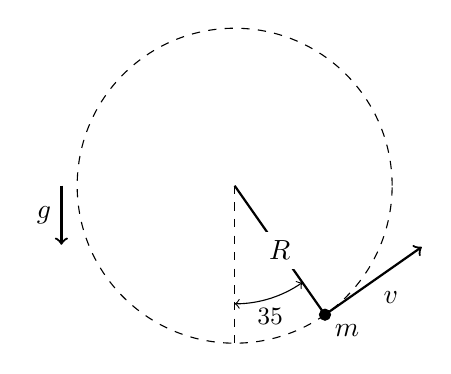
\begin{tikzpicture}
        \draw[dashed] (0,0) circle (2cm);
        \draw[thick,->] (180:2.2) -- ++(270:0.75cm)
            node[pos=0.5,anchor=east] {$g$};
        \draw[dashed] (0,0) -- (270:2cm);
        \draw[fill] (305:2) circle (2pt)
            node[anchor=north west] {$m$};
        \draw[thick,->] (305:2) -- ++(35:1.5cm)
            node[pos=0.5,anchor=north west] {$v$};
        \draw[thick] (0,0) -- (305:2)
            node[pos=0.5,fill=white,anchor=center] {$R$};
        \draw[<->] (270:1.5) arc (270:305:1.5)
            node[font=\small,pos=0.5,anchor=north] {\ang{35}};
    \end{tikzpicture}
    \end{center}
    When the string makes an angle of \ang{35} with the vertical as shown,
        the speed of the mass is \SI{5.0}{\meter\per\second}.
    At this instant what is the magnitude of the force the string exerts on the mass?
    \begin{multicols}{3}
    \begin{choices}
        \wrongchoice{\SI{50}{\newton}}
      \correctchoice{\SI{82}{\newton}}
        \wrongchoice{\SI{89}{\newton}}
        \wrongchoice{\SI{11}{\newton}}
        \wrongchoice{\SI{61}{\newton}}
    \end{choices}
    \end{multicols}
\end{question}
}

\element{serway-mc}{
\begin{question}{serway-ch06-q22}
    A split highway has a number of lanes for traffic. 
    For traffic going in one direction,
        the radius for the inside of the curve is half the radius for the outside.
    One car, car $A$, travels on the inside while another car of equal mass, car $B$,
        travels at equal speed on the outside of the curve. 
    Which statement about resultant forces on the cars is correct?
    \begin{choices}
        \wrongchoice{The force on $A$ is half the force on $B$.}
      \correctchoice{The force on $B$ is half the force on $A$.}
        \wrongchoice{The force on $A$ is four times the force on $B$.}
        \wrongchoice{The force on $B$ is four times the force on $A$.}
        \wrongchoice{There is no net resultant force on either as long as they stay on the road while turning.}
    \end{choices}
\end{question}
}

\element{serway-mc}{
\begin{question}{serway-ch06-q23}
    A race car traveling at \SI{100}{\meter\per\second} enters an unbanked turn of \SI{400}{\meter} radius. 
    The coefficient of (static) friction between the tires and the track is \num{1.1}. 
    The track has both an inner and an outer wall. 
    Which statement is correct?
    \begin{choices}
      \correctchoice{The race car will crash into the outer wall.}
        \wrongchoice{The race car will crash into the inner wall.}
        \wrongchoice{The car will stay in the center of the track.}
        \wrongchoice{The car will stay in the center of the track if the driver speeds up.}
        \wrongchoice{The car would stay in the center of the track if the radius were reduced to \SI{200}{\meter}.}
    \end{choices}
\end{question}
}

\element{serway-mc}{
\begin{question}{serway-ch06-q24}
    A student is sitting on the right side of a school bus when it makes a right turn.
    We know that the force of gravity acts downwards and a normal force from the seat acts upwards. 
    %% NOTE: added ``with respect to the bus''
    If the student stays in place with respect to the bus when the bus turns,
        we also know that there must be
    \begin{choices}
        \wrongchoice{no other force on the student.}
        \wrongchoice{a force parallel to the seat directed forward on the student.}
        \wrongchoice{a force parallel to the seat directed to the left on the student.}
      \correctchoice{a force parallel to the seat directed to the right on the student.}
        \wrongchoice{a force parallel to the seat in a direction between forward and left on the student.}
    \end{choices}
\end{question}
}

\element{serway-mc}{
\begin{question}{serway-ch06-q25}
    For a plane to be able to fly clockwise in a horizontal circle as seen from above,
        in addition to exerting a force downwards on the air:
    \begin{choices}
        \wrongchoice{it must be increasing its speed.}
      \correctchoice{it must exert a force on the air that is directed to the plane's left side.}
        \wrongchoice{it must exert a force on the air that is directed to the plane's right side.}
        \wrongchoice{it does not need to exert a force: it must only move the wing flaps out.}
        \wrongchoice{it only needs to deflect the air without exerting any additional force on the air.}
    \end{choices}
\end{question}
}

\element{serway-mc}{
\begin{question}{serway-ch06-q26}
    When a car goes around a circular curve on a level road,
    \begin{choices}
        \wrongchoice{no frictional force is needed because the car simply follows the road.}
        \wrongchoice{the frictional force of the road on the car increases when the car's speed decreases.}
      \correctchoice{the frictional force of the road on the car increases when the car's speed increases.}
        \wrongchoice{the frictional force of the road on the car increases when the car moves to the outside of the curve.}
        \wrongchoice{there is no net frictional force because the road and the car exert equal and opposite forces on each other.}
    \end{choices}
\end{question}
}

\element{serway-mc}{
\begin{question}{serway-ch06-q27}
    An iceboat is traveling in a circle on the ice. 
    Halfway around the circle the sail and the steering mechanism fall off the boat. 
    Which statement is correct?
    \begin{choices}
        \wrongchoice{The boat will continue traveling in the circle because there is no friction.}
        \wrongchoice{The boat will continue to travel in the circle because its velocity exerts a force on it.}
      \correctchoice{The boat will move off on a line tangent to the circle because there is no force on it.}
        \wrongchoice{The boat will move off tangent to the circle because there is a force on it perpendicular to the boat directed to the outside of the circle.}
        \wrongchoice{The boat will move off to the outside perpendicular to the tangent line since a force directed to the outside of the circle always acts on the boat.}
    \end{choices}
\end{question}
}

%% T: tension
%% F: force
%% N: normal force
\element{serway-mc}{
\begin{question}{serway-ch06-q28}
    A rock attached to a string swings in a vertical circle. 
    Which free body diagram could correctly describe the force(s)
        on the rock when it is at the highest point?
    \begin{multicols}{2}
    \begin{choices}
        \AMCboxDimensions{down=-1.0cm}
        \wrongchoice{
            \begin{tikzpicture}
                \draw[white] (-1,-1) rectangle (+1,+1);
                \draw[fill] (0,0) circle (1.5pt);
                \draw[very thick,->] (0,0) -- ++ (270:0.75) node[anchor=north] {$W$};
            \end{tikzpicture}
        }
        \wrongchoice{
            \begin{tikzpicture}
                \draw[white] (-1,-1) rectangle (+1,+1);
                \draw[fill] (0,0) circle (1.5pt);
                \draw[very thick,->] (0,0) -- ++ (90:0.50) node[anchor=west] {$N$};
                \draw[very thick,->] (0,0) -- ++ (270:0.75) node[anchor=north] {$W$};
            \end{tikzpicture}
        }
        %% ANS is C
        \correctchoice{
            \begin{tikzpicture}
                \draw[white] (-1,-1) rectangle (+1,+1);
                \draw[fill] (0,0) circle (1.5pt);
                \draw[very thick,->] (0.2,0) -- ++ (270:0.50) node[anchor=west] {$T$};
                \draw[very thick,->] (0,0) -- ++ (270:0.75) node[anchor=north] {$W$};
            \end{tikzpicture}
        }
        \wrongchoice{
            \begin{tikzpicture}
                \draw[white] (-1,-1) rectangle (+1,+1);
                \draw[fill] (0,0) circle (1.5pt);
                \draw[very thick,->] (0,0) -- ++ (270:0.75) node[anchor=north] {$T$};
            \end{tikzpicture}
        }
        \wrongchoice{
            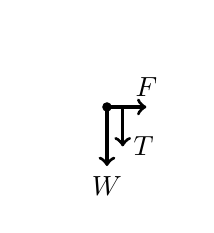
\begin{tikzpicture}
                \draw[white] (-1,-1) rectangle (+1,+1);
                \draw[fill] (0,0) circle (1.5pt);
                \draw[very thick,->] (0,0) -- ++ (0:0.5) node[anchor=south] {$F$};
                \draw[very thick,->] (0.2,0) -- ++ (270:0.50) node[anchor=west] {$T$};
                \draw[very thick,->] (0,0) -- ++ (270:0.75) node[anchor=north] {$W$};
            \end{tikzpicture}
        }
    \end{choices}
    \end{multicols}
\end{question}
}


%% NOTE: alternative question from Six Easy Lesson, p33
%% NOTE: include diagram of spinning object on string?
% A ball swings at the end of a string in a circular path in a vertical plane.
% Which free-body diagram best represents the forces acting on the ball when at the bottom of the circle and moving toward the right?
% The ball moves at constants speed.

\element{serway-mc}{
\begin{question}{serway-ch06-q29}
    A rock attached to a string swings in a vertical circle. 
    Which free body diagram could correctly describe the force(s) 
        on the rock when the string is in one possible horizontal position?
    \begin{multicols}{2}
    \begin{choices}
        \AMCboxDimensions{down=-0.8cm}
        \wrongchoice{
            \begin{tikzpicture}
                \draw[white] (-1,-1) rectangle (+1,+1);
                \draw[fill] (0,0) circle (1.5pt);
                \draw[very thick,->] (0,0) -- ++ (180:0.75) node[anchor=north] {$T$};
            \end{tikzpicture}
        }
        \wrongchoice{
            \begin{tikzpicture}
                \draw[white] (-1,-1) rectangle (+1,+1);
                \draw[fill] (0,0) circle (1.5pt);
                \draw[very thick,->] (0,0) -- ++ (270:0.75) node[anchor=north] {$W$};
            \end{tikzpicture}
        }
        %% ANS is C
        \correctchoice{
            \begin{tikzpicture}
                \draw[white] (-1,-1) rectangle (+1,+1);
                \draw[fill] (0,0) circle (1.5pt);
                \draw[very thick,->] (0,0) -- ++ (180:0.75) node[anchor=north west] {$T$};
                \draw[very thick,->] (0,0) -- ++ (270:0.75) node[anchor=north] {$W$};
            \end{tikzpicture}
        }
        \wrongchoice{
            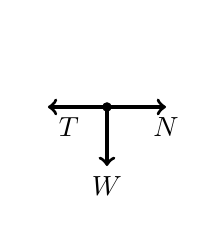
\begin{tikzpicture}
                \draw[white] (-1,-1) rectangle (+1,+1);
                \draw[fill] (0,0) circle (1.5pt);
                \draw[very thick,->] (0,0) -- ++ (180:0.75) node[anchor=north west] {$T$};
                \draw[very thick,->] (0,0) -- ++ (0:0.75) node[anchor=north] {$N$};
                \draw[very thick,->] (0,0) -- ++ (270:0.75) node[anchor=north] {$W$};
            \end{tikzpicture}
        }
        \wrongchoice{
            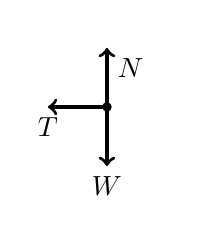
\begin{tikzpicture}
                \draw[white] (-1,-1) rectangle (+1,+1);
                \draw[fill] (0,0) circle (1.5pt);
                \draw[very thick,->] (0,0) -- ++ (180:0.75) node[anchor=north] {$T$};
                \draw[very thick,->] (0,0) -- ++ (90:0.75) node[anchor=north west] {$N$};
                \draw[very thick,->] (0,0) -- ++ (270:0.75) node[anchor=north] {$W$};
            \end{tikzpicture}
        }
    \end{choices}
    \end{multicols}
\end{question}
}

\element{serway-mc}{
\begin{question}{serway-ch06-q30}
    A rock attached to a string swings in a vertical circle. 
    Which free body diagram could correctly describe the force(s)
        on the rock when it is at the lowest point?
    \begin{multicols}{2}
    \begin{choices}
        \AMCboxDimensions{down=-1.0cm}
        \wrongchoice{
            \begin{tikzpicture}
                \draw[white] (-1,-1.5) rectangle (+1,+1.5);
                \draw[fill] (0,0) circle (1.5pt);
                \draw[very thick,->] (0,0) -- ++ (270:1) node[anchor=north] {$W$};
            \end{tikzpicture}
        }
        \correctchoice{
            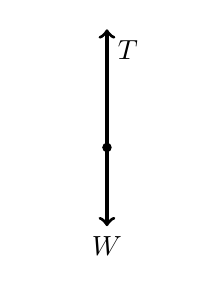
\begin{tikzpicture}
                \draw[white] (-1,-1.5) rectangle (+1,+1.5);
                \draw[fill] (0,0) circle (1.5pt);
                \draw[very thick,->] (0,0) -- ++ (270:1) node[anchor=north] {$W$};
                \draw[very thick,->] (0,0) -- ++ (90:1.5) node[anchor=north west] {$T$};
            \end{tikzpicture}
        }
        \wrongchoice{
            \begin{tikzpicture}
                \draw[white] (-1,-1.5) rectangle (+1,+1.5);
                \draw[fill] (0,0) circle (1.5pt);
                \draw[very thick,->] (0,0) -- ++ (90:1.5) node[anchor=north west] {$T$};
            \end{tikzpicture}
        }
        \wrongchoice{
            \begin{tikzpicture}
                \draw[white] (-1,-1.5) rectangle (+1,+1.5);
                \draw[fill] (0,0) circle (1.5pt);
                \draw[very thick,->] (0,0) -- ++ (270:1) node[anchor=north] {$N$};
                \draw[very thick,->] (0,0) -- ++ (90:1) node[anchor=north west] {$T$};
            \end{tikzpicture}
        }
        \wrongchoice{
            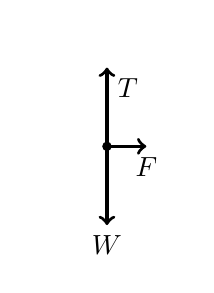
\begin{tikzpicture}
                \draw[white] (-1,-1.5) rectangle (+1,+1.5);
                \draw[fill] (0,0) circle (1.5pt);
                \draw[very thick,->] (0,0) -- ++ (0:0.5) node[anchor=north] {$F$};
                \draw[very thick,->] (0,0) -- ++ (270:1) node[anchor=north] {$W$};
                \draw[very thick,->] (0,0) -- ++ (90:1) node[anchor=north west] {$T$};
            \end{tikzpicture}
        }
    \end{choices}
    \end{multicols}
\end{question}
}

\element{serway-mc}{
\begin{question}{serway-ch06-q31}
    Two small cylindrical plastic containers with flat bottoms are placed on a turntable that has a smooth flat surface. 
    Canister $A$ is empty; canister $B$ contains lead shot. 
    Each canister is the same distance $r$ from the center. 
    The coefficient of static friction between the canisters and the turntable is $\mu_s$. 
    When the speed of the turntable is gradually increased,
    \begin{choices}
        \wrongchoice{only the lighter container slides outward off the turntable; the heavier one stays on.}
        \wrongchoice{only the heavier container slides outward off the turntable; the lighter one stays on.}
      \correctchoice{both containers slide off the turntable at the same turntable speed.}
        \wrongchoice{the lighter container slides inward.}
        \wrongchoice{the heavier container slides inward.}
    \end{choices}
\end{question}
}

\element{serway-mc}{
\begin{question}{serway-ch06-q32}
    A hornet circles around a pop can at increasing speed while
        flying in a path with a \SI{12}{\centi\meter} diameter. 
    We can conclude that the hornet's wings must push on the air
        with force components that are
    \begin{choices}
        \wrongchoice{straight down.}
        \wrongchoice{down and inwards.}
      \correctchoice{down and outwards.}
        \wrongchoice{down and backwards.}
        \wrongchoice{down, inwards and backwards.}
    \end{choices}
\end{question}
}

\element{serway-mc}{
\begin{question}{serway-ch06-q33}
    A hornet circles around a pop can at constant speed once per second in a path with a \SI{12}{\centi\meter} diameter. 
    We can conclude that the hornet's wings must push on the air with force components that are:
    \begin{choices}
        \wrongchoice{straight down.}
        \wrongchoice{down and inwards.}
        \wrongchoice{down and outwards.}
        \wrongchoice{down and backwards.}
      \correctchoice{down, backwards and outwards.}
    \end{choices}
\end{question}
}

\element{serway-mc}{
\begin{question}{serway-ch06-q34}
    Frank says that if you release the string when swinging a ball in a horizontal circle,
        the ball flies out in the radial direction defined by the string at the instant you release the ball. 
    John says that it flies out along a tangent line perpendicular to the string,
        and that it then drops straight down to the ground. 
    Which one, if either, is correct?
    \begin{choices}
        \wrongchoice{Frank, because the centrifugal force is no longer counteracted by the string.}
        \wrongchoice{Frank, because balls naturally fly straight out.}
        \wrongchoice{John, because there is no centrifugal force.}
        \wrongchoice{John, because balls fall straight down when released.}
      \correctchoice{Neither, because although there is no centrifugal force, and the ball's velocity is tangent to the circle at the instant of release, the ball then follows a parabolic trajectory.}
    \end{choices}
\end{question}
}

\element{serway-mc}{
\begin{question}{serway-ch06-q35}
    The equation below is the solution to a problem.
    \begin{align*}
        & \dfrac{\left(\SI{2.00}{\kilo\gram}\right)\left(\SI{8.00}{\meter\per\second\squared}\right)^2}{\left(\SI{5.00}{\meter}\right)} = \\
        &\quad\quad \SI{6.00}{\newton} - \left(\SI{2.00}{\kilo\gram}\right)\left(\SI{9.8}{\meter\per\second\squared}\right)\left(\cos\ang{180}\right)
    \end{align*}
    The best physical representation of this equation is:
    \begin{choices}
        \wrongchoice{a sphere of \SI{2.00}{\kilo\gram} mass under a \SI{6.00}{\newton} tension when at the bottom of a vertical circle.}
        \wrongchoice{a sphere of \SI{2.00}{\kilo\gram} mass under a \SI{6.00}{\newton} tension when at the side of a vertical circle.}
      \correctchoice{a sphere of \SI{2.00}{\kilo\gram} mass under a \SI{6.00}{\newton} tension when at the top of a vertical circle.}
        \wrongchoice{a sphere of \SI{2.00}{\kilo\gram} mass at any point on a horizontal circle.}
        \wrongchoice{a \SI{2.00}{\kilo\gram} gecko running on the ceiling with a speed of \SI{8.00}{\meter\per\second}.}
    \end{choices}
\end{question}
}

\element{serway-mc}{
\begin{question}{serway-ch06-q36}
    The equation below is the solution to a problem.
    \begin{align*}
        & \dfrac{\left(\SI{2.00}{\kilo\gram}\right)\left(\SI{8.00}{\meter\per\second\squared}\right)^2}{\left(\SI{5.00}{\meter}\right)} = \\
        &\quad\quad = \SI{6.00}{\newton} - \left(\SI{2.00}{\kilo\gram}\right)\left(\SI{9.8}{\meter\per\second\squared}\right)\left(\cos\ang{0}\right)
    \end{align*}
    The best physical representation of this equation is:
    \begin{choices}
      \correctchoice{a sphere of \SI{2.00}{\kilo\gram} mass under a \SI{6.00}{\newton} tension when at the bottom of a vertical circle.}
        \wrongchoice{a sphere of \SI{2.00}{\kilo\gram} mass under a \SI{6.00}{\newton} tension when at the side of a vertical circle.}
        \wrongchoice{a sphere of \SI{2.00}{\kilo\gram} mass under a \SI{6.00}{\newton} tension when at the top of a vertical circle.}
        \wrongchoice{a sphere of \SI{2.00}{\kilo\gram} mass at any point on a horizontal circle.}
        \wrongchoice{a \SI{2.00}{\kilo\gram} gecko running on the ceiling with a speed of \SI{8.00}{\meter\per\second}.}
    \end{choices}
\end{question}
}

\element{serway-mc}{
\begin{question}{serway-ch06-q37}
    The equation below is the solution to a problem.
    \begin{align*}
        & \dfrac{\left(\SI{2.00}{\kilo\gram}\right)\left(\SI{8.00}{\meter\per\second\squared}\right)^2}{\left(\SI{5.00}{\meter}\right)} = \\
        &\quad\quad \SI{6.00}{\newton} - \left(\SI{2.00}{\kilo\gram}\right)\left(\SI{9.8}{\meter\per\second\squared}\right)\left(\cos\ang{90}\right)
    \end{align*}
    The best physical representation of this equation is:
    \begin{choices}
        \wrongchoice{a sphere of \SI{2.00}{\kilo\gram} mass under a \SI{6.00}{\newton} tension when at the bottom of a vertical circle.}
      \correctchoice{a sphere of \SI{2.00}{\kilo\gram} mass under a \SI{6.00}{\newton} tension when at the side of a vertical circle.}
        \wrongchoice{a sphere of \SI{2.00}{\kilo\gram} mass under a \SI{6.00}{\newton} tension when at the top of a vertical circle.}
        \wrongchoice{a sphere of \SI{2.00}{\kilo\gram} mass at any point on a horizontal circle.}
        \wrongchoice{a \SI{2.00}{\kilo\gram} gecko running on the ceiling with a speed of \SI{8.00}{\meter\per\second}.}
    \end{choices}
\end{question}
}

\element{serway-mc}{
\begin{question}{serway-ch06-q38}
    The coefficient of static friction for the tires of a race car is \num{0.950} and the coefficient of kinetic friction is \num{0.800}. 
    The car is on a level circular track of \SI{50.0}{\meter} radius on a planet where $g=\SI{2.45}{\meter\per\second\squared}$ compared to Earth's $g=\SI{9.80}{\meter\per\second\squared}$.
    The maximum safe speed on the track on the planet is \rule[-0.1pt]{4em}{0.1pt} times as large as the maximum safe speed on Earth.
    \begin{multicols}{3}
    \begin{choices}
        \wrongchoice{\num{0.25}}
      \correctchoice{\num{0.50}}
        \wrongchoice{\num{1.00}}
        \wrongchoice{\num{2.00}}
        \wrongchoice{\num{4.00}}
    \end{choices}
    \end{multicols}
\end{question}
}

\element{serway-mc}{
\begin{question}{serway-ch06-q39}
    The coefficient of static friction for the tires of a race car is \num{0.950} and the coefficient of kinetic friction is \num{0.800}. 
    The car is on a level circular track of \SI{50.0}{\meter} radius on a planet where $g=\SI{2.45}{\meter\per\second\squared}$ compared to Earth's $g=\SI{9.80}{\meter\per\second\squared}$.
    If the car is to be able to travel at the same speed on the planet as on Earth,
        the radius of the track on the planet must be \rule[-0.1pt]{4em}{0.1pt} times as large as the radius of the track on Earth.
    \begin{multicols}{3}
    \begin{choices}
        \wrongchoice{\num{0.25}}
        \wrongchoice{\num{0.50}}
        \wrongchoice{\num{1.00}}
        \wrongchoice{\num{2.00}}
      \correctchoice{\num{4.00}}
    \end{choices}
    \end{multicols}
\end{question}
}

\element{serway-mc}{
\begin{question}{serway-ch06-q40}
    A boy on board a cruise ship drops a \SI{30.0}{\gram} marble into the ocean. 
    If the resistive force proportionality constant is \SI{0.500}{\kilo\gram\per\second},
        what is the terminal speed of the marble?
    \begin{multicols}{2}
    \begin{choices}
        \wrongchoice{\SI{0.147}{\meter\per\second}}
        \wrongchoice{\SI{0.294}{\meter\per\second}}
      \correctchoice{\SI{0.588}{\meter\per\second}}
        \wrongchoice{\SI{1.18}{\meter\per\second}}
        \wrongchoice{\SI{2.35}{\meter\per\second}}
    \end{choices}
    \end{multicols}
\end{question}
}

\element{serway-mc}{
\begin{question}{serway-ch06-q41}
    In a recent mystery,
        the hero saves himself by spreading out a windshield tarpaulin to reduce his terminal velocity. 
    A skydiver of \SI{75}{\kilo\gram} mass has a terminal velocity of \SI{60}{\meter\per\second}.
    If the hero has the same \SI{75}{\kilo\gram} mass,
        the same density as the sky diver,
        and a drag coefficient twice as large with the tarp,
        by what factor is his effective area greater than the \SI{0.70}{\meter\squared} area of the skydiver?
    \begin{multicols}{3}
    \begin{choices}
        \wrongchoice{\num{4}}
        \wrongchoice{\num{8}}
        \wrongchoice{\num{16}}
      \correctchoice{\num{32}}
        \wrongchoice{\num{64}}
    \end{choices}
    \end{multicols}
\end{question}
}

\element{serway-mc}{
\begin{question}{serway-ch06-q42}
    The following equation was obtained by solving a physics problem:
    \begin{equation*}
        \dfrac{\left(\SI{16.0}{\meter\per\second}\right)^2}
              {\left(\SI{75.0}{\meter}\right)\left(\SI{9.80}{\meter\per\second\squared}\right)}
          = \tan\ang{19.2}
    \end{equation*}
    The best physical representation of the situation is:
    \begin{choices}
        \wrongchoice{A car traveling at \SI{16.0}{\meter\per\second} is \ang{19.2} into a turn of a quarter circle on a level road.}
        \wrongchoice{A mass on a string that is originally horizontal has fallen to where the angle between the string and the vertical direction is \ang{19.2}.}
        \wrongchoice{A mass on a string originally horizontal has fallen \ang{19.2} from the horizontal direction.}
      \correctchoice{A car traveling at \SI{16.0}{\meter\per\second} is on a circular curve banked at \ang{19.2}.}
        \wrongchoice{A car traveling at \SI{16.0}{\meter\per\second} and going over a semicircular mountain-top road is \ang{19.2} down from the top.}
    \end{choices}
\end{question}
}

\element{serway-mc}{
\begin{question}{serway-ch06-q43}
    An airplane flies in a horizontal circle of radius \SI{500}{\meter}
        at a speed of \SI{150}{\meter\per\second}.
    If the plane were to fly in the same \SI{500}{\meter} circle
        at a speed of \SI{300}{\meter\per\second},
        by what factor would its centripetal acceleration change?
    \begin{multicols}{3}
    \begin{choices}
        \wrongchoice{\num{0.25}}
        \wrongchoice{\num{0.50}}
        \wrongchoice{\num{1.00}}
        \wrongchoice{\num{2.00}}
      \correctchoice{\num{4.00}}
    \end{choices}
    \end{multicols}
\end{question}
}

\element{serway-mc}{
\begin{question}{serway-ch06-q44}
    An airplane flies in a horizontal circle of radius \SI{500}{\meter}
        at a speed of \SI{150}{\meter\per\second}.
    If the radius were changed to \SI{1000}{\meter},
        but the speed remained the same,
        by what factor would its centripetal acceleration change?
    \begin{multicols}{3}
    \begin{choices}
        \wrongchoice{\num{0.25}}
      \correctchoice{\num{0.50}}
        \wrongchoice{\num{1.00}}
        \wrongchoice{\num{2.00}}
        \wrongchoice{\num{4.00}}
    \end{choices}
    \end{multicols}
\end{question}
}

\element{serway-mc}{
\begin{question}{serway-ch06-q45}
    An airplane flies in a horizontal circle of radius \SI{500}{\meter}
        at a speed of \SI{150}{\meter\per\second}.
    %% changed wording, removed ``same''
    If the radius were changed to \SI{1000}{\meter},
        and the speed to \SI{300}{\meter\per\second},
        by what factor would its centripetal acceleration change?
    \begin{multicols}{3}
    \begin{choices}
        \wrongchoice{\num{0.25}}
        \wrongchoice{\num{0.50}}
        \wrongchoice{\num{1.00}}
      \correctchoice{\num{2.00}}
        \wrongchoice{\num{4.00}}
    \end{choices}
    \end{multicols}
\end{question}
}

\element{serway-mc}{
\begin{question}{serway-ch06-q46}
    A car enters a level,
        unbanked semi-circular hairpin turn of \SI{100}{\meter}
        radius at a speed of \SI{28}{\meter\per\second}. 
    The coefficient of friction between the tires and the road is $\mu=\num{0.800}$.
    If the car maintains a constant speed of \SI{28}{\meter\per\second},
        it will:
    \begin{choices}
        \wrongchoice{attempt to dig into the road surface.}
        \wrongchoice{tend to veer toward the center of the semicircle.}
      \correctchoice{arrive safely at the end of the semicircle.}
        \wrongchoice{tend to veer toward the outside of the circle.}
        \wrongchoice{veer toward the center for the first quarter-circle, then veer toward the outside for the second quarter-circle.}
    \end{choices}
\end{question}
}

\element{serway-mc}{
\begin{question}{serway-ch06-q47}
    A car enters a level,
        unbanked semi-circular hairpin turn of \SI{100}{\meter}
        radius at a speed of \SI{40}{\meter\per\second}. 
    The coefficient of friction between the tires and the road is $\mu=\num{0.25}$.
    If the car maintains a constant speed of \SI{40}{\meter\per\second},
        it will:
    \begin{choices}
        \wrongchoice{attempt to dig into the road surface.}
        \wrongchoice{tend to veer toward the center of the semicircle.}
        \wrongchoice{arrive safely at the end of the semicircle.}
      \correctchoice{tend to veer toward the outside of the circle.}
        \wrongchoice{veer toward the center for the first quarter-circle, then veer toward the outside for the second quarter-circle.}
    \end{choices}
\end{question}
}

\endinput


